\chapter{Estimating the luminosity}
\section{Concept of luminosity}
In particle physics experiments, the energy available for producing new effects is a crucial parameter. This energy is determined by the centre of mass energy, which can be optimized through colliding beams, minimizing energy loss in the motion of the centre of mass system. Another critical aspect is the number of useful interactions or events, especially when studying rare events with a small production cross-section $\sigma_p$. The ability of a particle accelerator to produce the required number of interactions is quantified by the concept of luminosity, defined as the proportionality factor between the number of events per second $\tfrac{dR}{dt}$ and the cross-section. The relation between luminosity $\mathcal{L}$, cross-section $\sigma_p$ and ratio $\tfrac{dR}{dt}$ is defined as:
\begin{equation}
    \frac{dR}{dt} = \mathcal{L}{\sigma_p}
\end{equation}
The unit of luminosity is therefore $\SI{}{\per\centi\meter\squared\per\second}$
\paragraph{Luminosity in Fixed Target Experiments}
In fixed target experiments, the luminosity is influenced by the properties of both the incoming beam and the stationary target. The incoming beam is characterized by its flux $\Phi$, which is the number of particles per second. The target is described by its density $\rho_T$ and its length $l$. The luminosity in this setup is calculated using the formula:

\[
\mathcal{L}_{FT} = \Phi \cdot \rho_T \cdot l
\]

Given this definition, the interaction rate can be expressed as:

\[
\frac{dR}{dt} = \Phi \cdot \rho_T \cdot l \cdot \sigma_p
\]

\paragraph{Luminosity in Colliding Beam Experiments}
In colliding beam experiments, both beams act as the target and the incoming beam simultaneously. The general expression for luminosity in this case involves the convolution of the 3-D distribution functions of the beams, considering the overlap integral. A schematic picture is shoen in Figure \ref{fig:lumi-def}. Since the two beams are not stationary but moving through each other, the overlap integral depends on the longitudinal position of the bunches and therefore on the time as they move towards and through each other. For our integration we use the distance of the two beams to the central collision point $s_0 = ct$ as the ”time” variable. 
The luminosity is proportional to the overlap integral of the two  $\rho_1$, $\rho_2$ time dependent beam density distribution function:

\begin{figure}
    \centering
    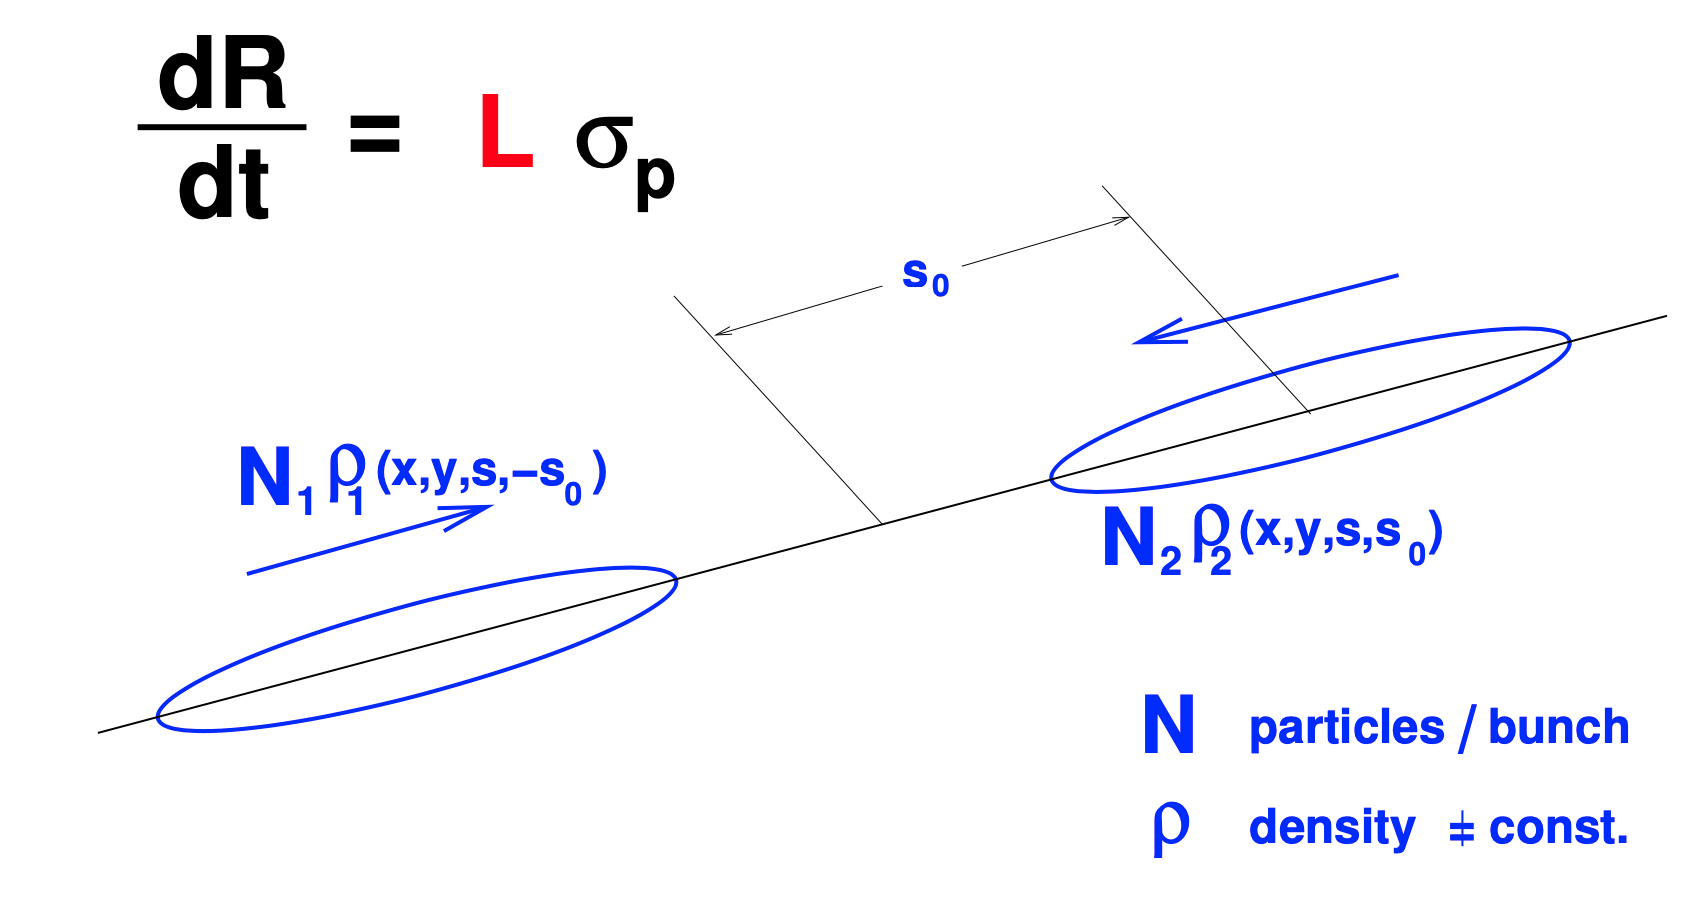
\includegraphics[width=0.6\textwidth]{figures/luminosity_def.png}
    \caption{Schematic view of a colliding beam interaction.}
    \label{fig:lumi-def}
\end{figure}

\begin{equation}
    \mathcal{L} \propto K\cdot\int\int\int\int_{-\infty}^{+\infty}\rho_1(x,y,s,s_0)\rho_2(x,y,s,s_0)dxdydsds_0.
\end{equation}

Assuming colliding bunches moving against each other that meet at $s_0$, we have to take into account the kinematic factor:
\begin{equation}
    K = \sqrt{\bigl(\vec{v_1}-\vec{v_2}\bigr)^2-\bigl(\vec{v_1} \times \vec{v_2}\bigr)^2/c^2}.
\end{equation}
By further assuming head-on collisions ($\vec{v_1}=-\vec{v_2}$) and that all densities are uncorrelated in all planes, we can write:
\begin{equation}
        \mathcal{L} = 2 N_1 N_2 f N_b\cdot\int\int\int\int_{\infty}^{+\infty}\rho_{1x}(x)\rho_{1y}(y)\rho_{1s}(s+s_0)\rho_{2x}(x)\rho_{2y}(y)\rho_{2s}(s+s_0)dxdydsds_0.
\end{equation}
\[
\mathcal{L} = 2 \cdot N_1 \cdot N_2 \cdot f \cdot N_b \cdot \frac{1}{(2 \pi)^{3/2} \sigma_x \sigma_y \sigma_s}
\]

where:
\begin{itemize}
    \item \( N_1 \) and \( N_2 \) are the number of particles per bunch for each beam.
    \item \( f \) is the revolution frequency.
    \item \( N_b \) is the number of bunches in each beam.
\end{itemize}

To evaluate this integral one should know all distributions. An analytical calculation is not always possible and a numerical integration may be required. However in many cases the beams follow ”reasonable” profiles and we can obtain closed solutions.


Concept of luminosity,  Werner Herr and Bruno Muratori\\
Luminosity and luminous region shape for pure Gaussian bunches, M. Ferro-Luzzi, CERN, Geneva, Switzerland LHCb Public Note LHCb-PUB-2012-016

\section{Luminometers at LHCb}
\textit{Brief excursus on the available luminometers we have at LHCb. PLUME but also all the other online/offline counters, etc.}
\section{An absolute luminosity calibration: The Van Der Meer scan}
\textit{Explaination of what VdM is and how we use it to calibrate luminosity.}\\
Van der Meer scan luminosity measurement and beam–beam correction, Vladislav Balagura

\section{Combining the counters for a single luminosity measurement}
\textit{How we combine the 208 available measurements of luminosity: study on which estimator to choose between mean, median and trimmed mean}